%


\documentclass[twoside]{article}
\setlength{\oddsidemargin}{0.25 in}
\setlength{\evensidemargin}{-0.25 in}
\setlength{\topmargin}{-0.6 in}
\setlength{\textwidth}{6.5 in}
\setlength{\textheight}{8.5 in}
\setlength{\headsep}{0.75 in}
\setlength{\parindent}{0 in}
\setlength{\parskip}{0.1 in}

%
% ADD PACKAGES here:
%

\usepackage{amsmath,amsfonts,graphicx}

%
\newcounter{lecnum}
\renewcommand{\thepage}{\thelecnum-\arabic{page}}
\renewcommand{\thesection}{\thelecnum.\arabic{section}}
\renewcommand{\theequation}{\thelecnum.\arabic{equation}}
\renewcommand{\thefigure}{\thelecnum.\arabic{figure}}
\renewcommand{\thetable}{\thelecnum.\arabic{table}}

%
% The following macro is used to generate the header.
%
\newcommand{\lecture}[4]{
   \pagestyle{myheadings}
   \thispagestyle{plain}
   \newpage
   \setcounter{lecnum}{#1}
   \setcounter{page}{1}
   \noindent
   \begin{center}
   \framebox{
      \vbox{\vspace{2mm}
    \hbox to 6.28in { {\bf EE302 - Feedback Systems
	\hfill Spring 2019} }
       \vspace{4mm}
       \hbox to 6.28in { {\Large \hfill Lecture #1 \hfill} }
       \vspace{2mm}
       \hbox to 6.28in { {\it Lecturer: #2 \hfill } }
      \vspace{2mm}}
   }
   \end{center}
   \markboth{Lecture #1}{Lecture #1}

   \vspace*{4mm}
}
%
\renewcommand{\cite}[1]{[#1]}
\def\beginrefs{\begin{list}%
        {[\arabic{equation}]}{\usecounter{equation}
         \setlength{\leftmargin}{2.0truecm}\setlength{\labelsep}{0.4truecm}%
         \setlength{\labelwidth}{1.6truecm}}}
\def\endrefs{\end{list}}
\def\bibentry#1{\item[\hbox{[#1]}]}

%Use this command for a figure; it puts a figure in wherever you want it.
%usage: \fig{NUMBER}{SPACE-IN-INCHES}{CAPTION}
\newcommand{\fig}[3]{
			\vspace{#2}
			\begin{center}
			Figure \thelecnum.#1:~#3
			\end{center}
	}
% Use these for theorems, lemmas, proofs, etc.
\newtheorem{theorem}{Theorem}[lecnum]
\newtheorem{lemma}[theorem]{Lemma}
\newtheorem{proposition}[theorem]{Proposition}
\newtheorem{claim}[theorem]{Claim}
\newtheorem{corollary}[theorem]{Corollary}
\newtheorem{definition}[theorem]{Definition}
\newenvironment{proof}{{\bf Proof:}}{\hfill\rule{2mm}{2mm}}

% **** IF YOU WANT TO DEFINE ADDITIONAL MACROS FOR YOURSELF, PUT THEM HERE:

\begin{document}

% Lecture Details
\lecture{14}{Asst. Prof. M. Mert Ankarali}

\par

\section{Frequency Response Techniques in Control Systems}

Let's assume $u(t)$, $y(t)$, and $G(t)$ represents the input, output,
and transfer function representation of an input-output continuous time
system.

In order to characterize frequency response of a dynamical system,
the test signal is 
%
\begin{align*}
 u(t) = e^{j \omega t}
\end{align*}
%
which is an artificial complex periodic signal with a 
frequency of $\omega$. The Laplace transform of $u(t)$ takes the
form
%
\begin{align*}
 U(s) = \mathcal{L} \lbrace e^{j \omega t} \rbrace = \frac{1}{s - j \omega}
\end{align*}
%
Response of the system in s-domain is given by
%
%
\begin{align*}
 Y(s) = G(s) U(s) = G(s) \frac{1}{s - j \omega}
\end{align*}
%
Assuming that $G(s)$ is a rational transfer function
we can perform a partial fraction expansion
%
\begin{align*}
     Y(s) &= \frac{a}{s -  j \omega} + \left[ \mathrm{terms \ due \
  to \ the \ poles \ of} \  G(s) \right] 
\\
a &= \lim_{s \to j \omega} \left[ (s - j \omega) Y(s)
  \right]  = G(j \omega)
\\
Y(s) &=  \frac{G(j \omega)}{s -  j \omega} + \left[ \mathrm{terms \ due \
  to \ the \ poles \ of} \  G(s) \right]  
\end{align*}
%
Taking the inverse Laplace transform yields
%
\begin{align*}
  y(t) = G(j \omega) e^{j \omega t} + \mathcal{L}^{-1} \left[ \mathrm{terms \ due \
  to \ the \ poles \ of} \  G(s) \right]  
\end{align*}
%
If we assume that the system is ``stable'' or system is a part of
closed loop system and closed loop behavior is stable then
at steady state we have
%
\begin{align*}
y_{ss}(t) &= G(j \omega) e^{j \omega t} \\
&= | G(j \omega) | e^{i \omega t + \angle [ G(j \omega) ] }
\\
&= M e^{i \omega t + \theta}
\end{align*}
%
In other words complex periodic signal is scaled and phase shifted
based on the following operators
%
\begin{align*}
M &= | G(j \omega) | \\
\theta &= \angle G(j \omega)
\end{align*}
%
It is very easy to show that for a general real time domain signal
$u(t) = \sin (\omega t + \phi)$, the output $y(t)$ at steady state 
is computed via
%
\begin{align*}
  y_{ss}(t) = M \sin(\omega t + \phi + \theta)
\end{align*}
%

\newpage

\subsection{Plotting Frequency Response: Polar Plot}

We can consider the frequency response function $G(j \omega)$
as a mapping from positive $j \omega$ axis to a curve in 
the complex plane. In polar plot, we draw the frequency response
function starting from $\omega = 0$ (or $\omega \to 0^+$) to $\omega
\to \infty$.

Let's draw the polar plots of 
%
\begin{align*}
 G_1(s) &= s
 \quad , \quad
 G_2(s) = \frac{1}{s}
 \quad , \quad
 G_3(s) = s + 2
\\
 G_4(s) &= 2 + \frac{1}{s}
\quad , \quad
 G_5(s) = 2 + s +  \frac{1}{s}
\end{align*}

\vspace{6 pt}

  \begin{minipage}[h]{1\linewidth}
    \begin{center}
      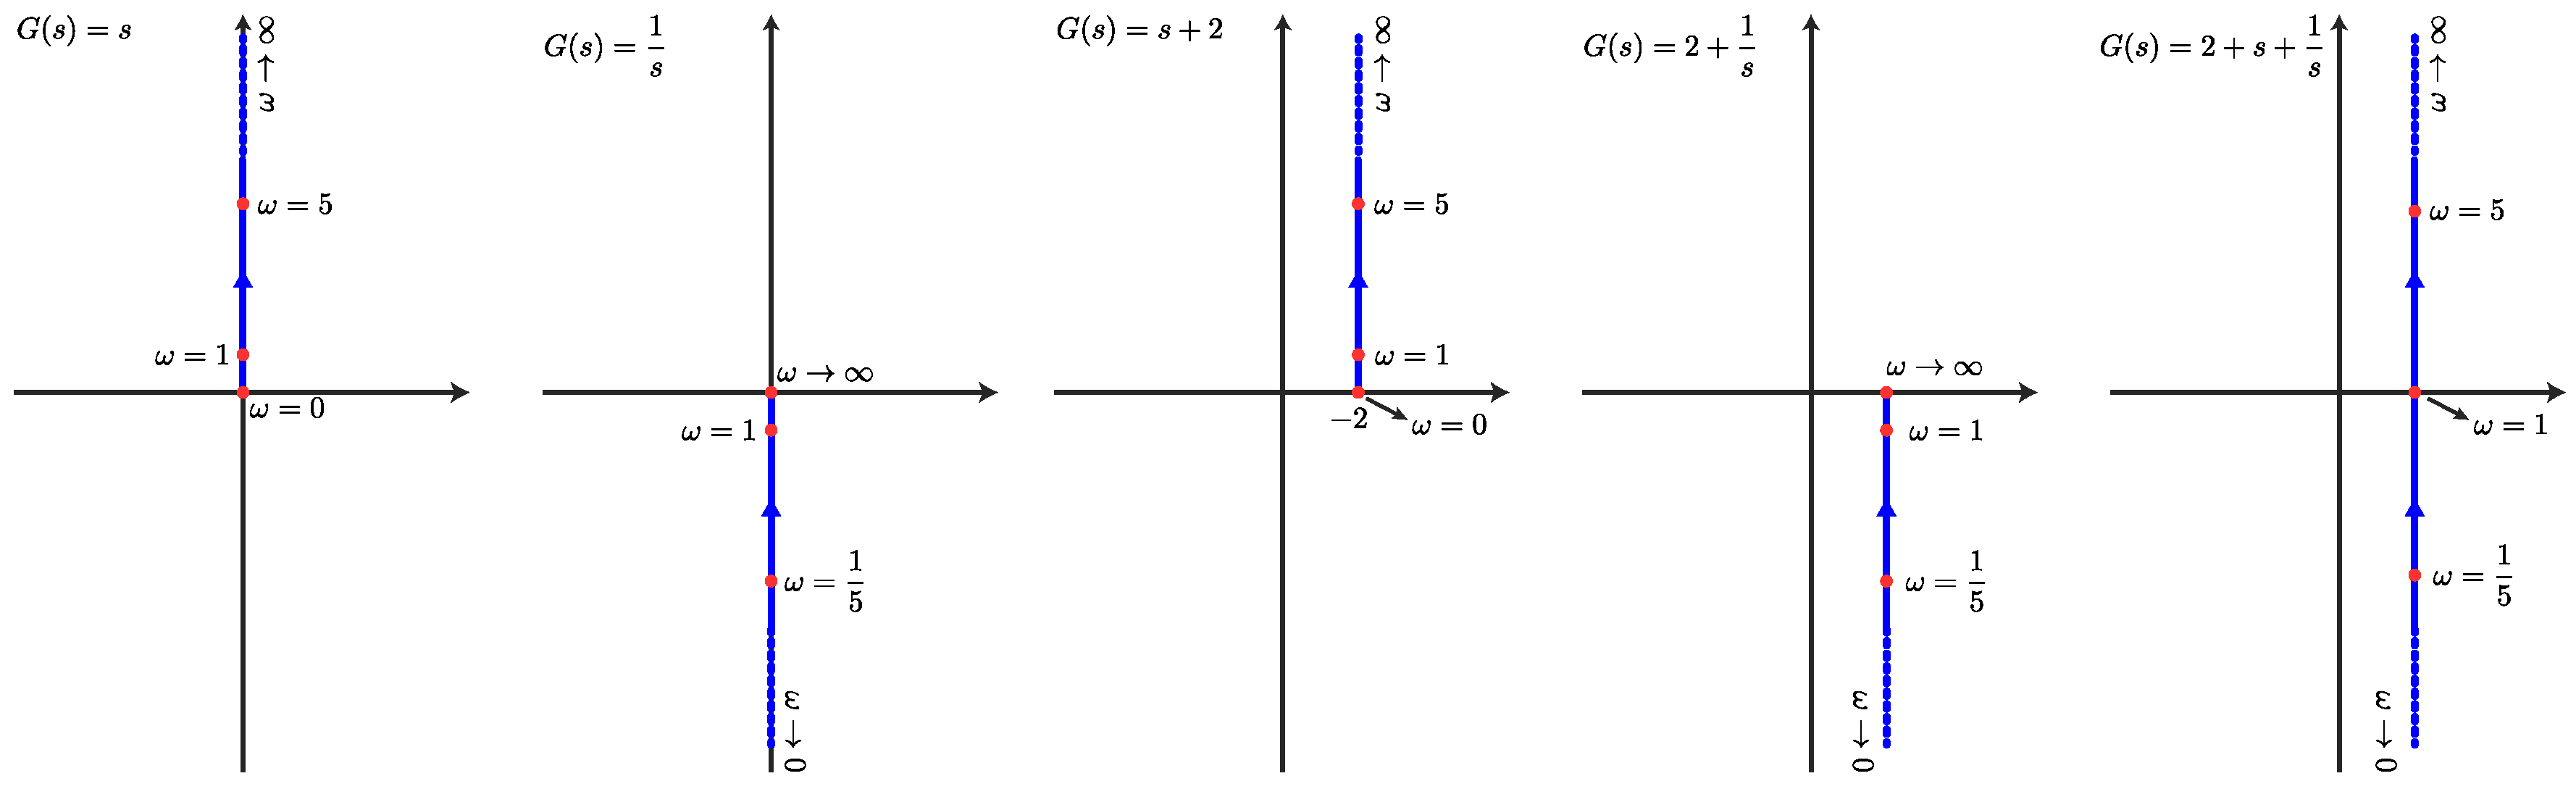
\includegraphics[width=0.99\textwidth]{polar}
    \end{center}
  \end{minipage}

\vspace{6 pt}

Now let's draw the polar plots of 
%
\begin{align*}
 G_1(s) &= \frac{1}{s+1}
 \quad , \quad
 G_2(s) = \frac{s}{s+1}
\end{align*}

Let's analyze $G_1(j \omega)$ for $\omega \in [0 , \infty)$

\begin{align*}
 G_1(j \omega) &= \frac{1}{j \omega +1} = \frac{1 - j \omega}{\omega^2 +1} 
= \frac{1}{\omega^2 +1} - \frac{\omega}{\omega^2 +1} j
\\
| G_1(j \omega) | &= \frac{1}{ \sqrt{1 + \omega^2} }
\\
\angle [ G_1(j \omega) ] &= \arctan (-\omega) 
\end{align*}

Now let's analyze $G_2(j \omega)$ for $\omega \in [0 , \infty)$

\begin{align*}
 G_2(j \omega) &= \frac{j \omega}{j \omega +1} = \frac{j \omega + \omega^2}{\omega^2 +1} 
= \frac{\omega^2}{\omega^2 +1} + \frac{\omega}{\omega^2 +1} j
\\
| G_2(j \omega) | &= \sqrt{ \frac{ \omega^2 }{ 1 + \omega^2 } }
\\
\angle [ G_2(j \omega) ] &= \arctan (1 / \omega) 
\end{align*}

Polar plots of $G_1(s)$ and $G_2(s)$ are illustrated below. 

\vspace{6 pt}

  \begin{minipage}[h]{1\linewidth}
    \begin{center}
      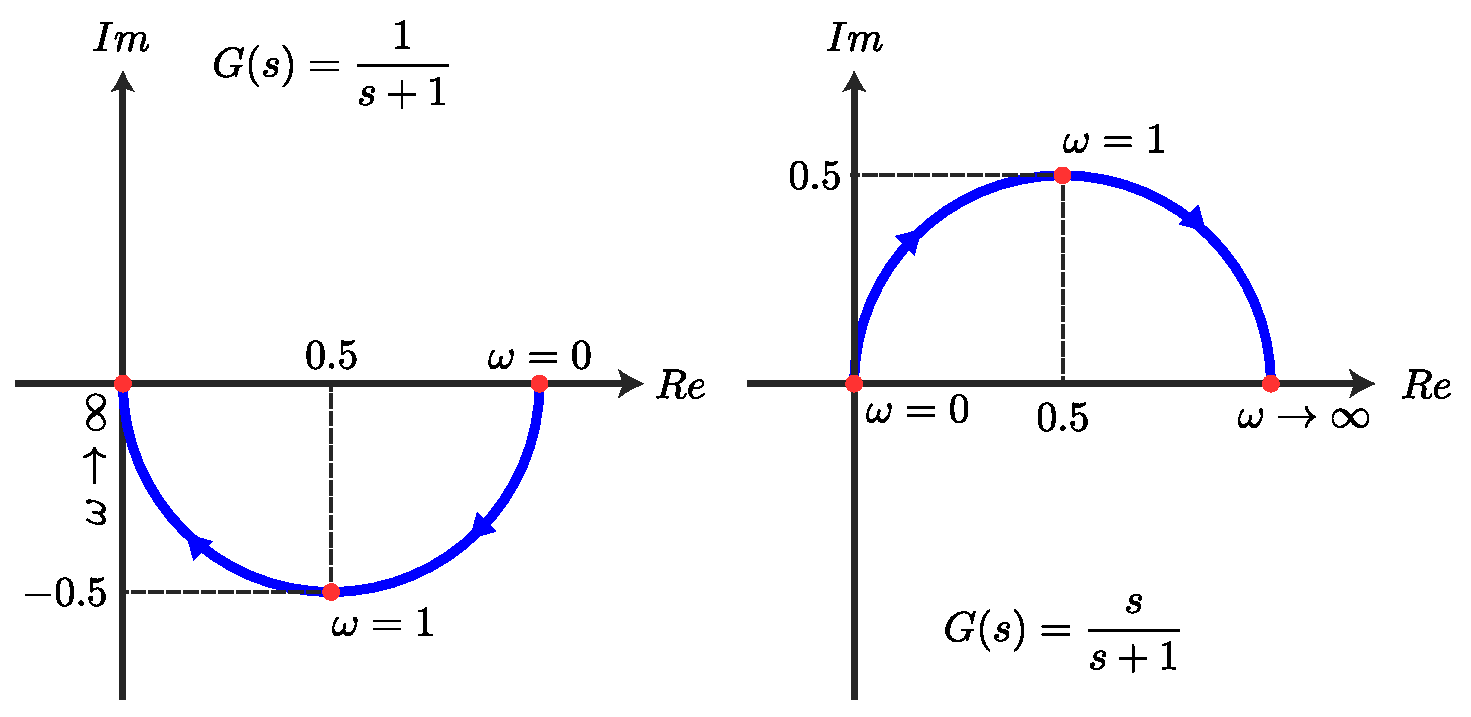
\includegraphics[width=0.9\textwidth]{polar2}
    \end{center}
  \end{minipage}

\vspace{6 pt}

Now let's draw the polar plot of  $G(s) = \frac{s - 1}{s+1}$ (note that
there is a zero in open-right half plane). Note that 
%
\begin{align*}
  G(s) &= 1 - \frac{2}{s+1}
  \\
  G(j \omega) &= 1 - 2 \left( \frac{1}{\omega^2 +1} - \frac{\omega}{\omega^2 +1} j \right)
\end{align*}

Process of polar plot drawing of $G(s) = \frac{s - 1}{s+1}$ is illustrated
below

\vspace{6 pt}

  \begin{minipage}[h]{1\linewidth}
    \begin{center}
      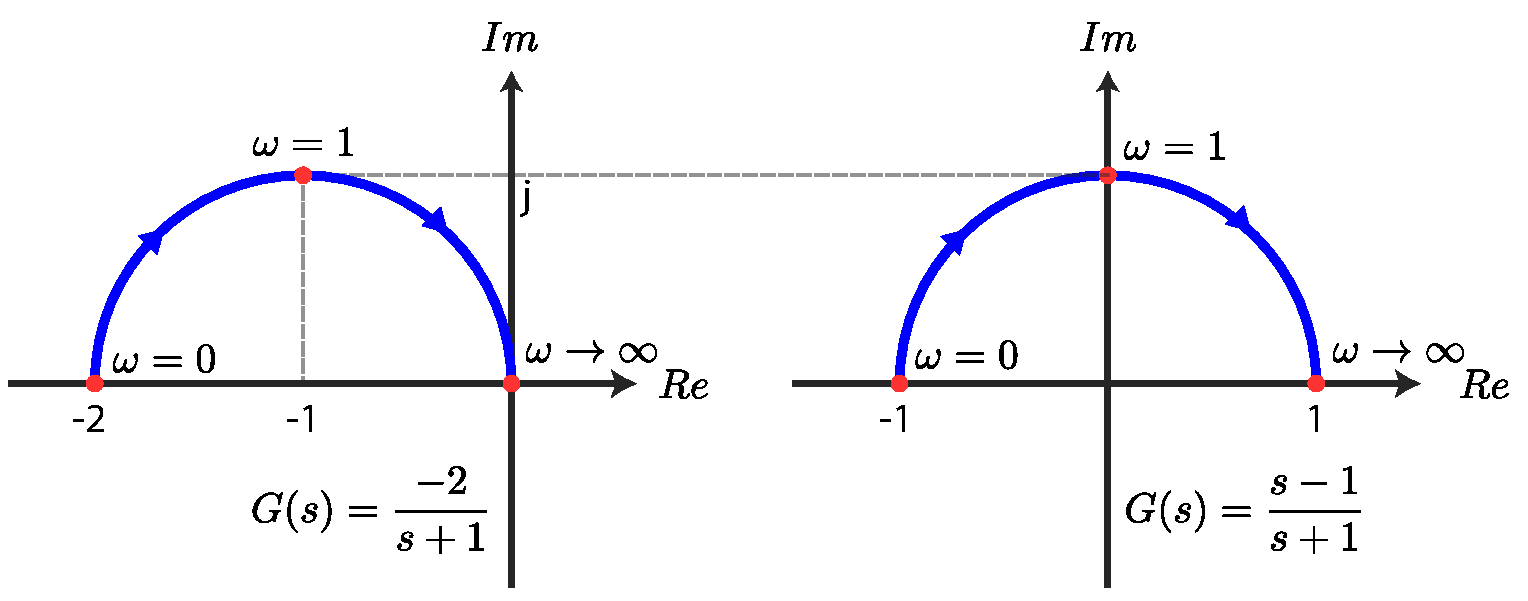
\includegraphics[width=0.9\textwidth]{polar3}
    \end{center}
  \end{minipage}

\vspace{6 pt}

Now let's draw the polar plot of  $G(s) = \frac{1}{(s+1)^2}$
%
\begin{align*}
  G(j \omega ) &= \frac{1}{ (j \omega + 1)^2 } = \frac{ (-j \omega + 1)^2 }{( \omega^2 +1 )^2 }
\\
&= \left[ \left( 1 - \omega^2 \right) + j ( - 2 \omega) \right] \frac{1}{( \omega^2 +1 )^2 }
\end{align*}
%
Some important points and associated features on the polar plot can be computed as
\begin{align*}
  \omega &\to 0 \ \Rightarrow G(j \omega) = 1
\\
 \omega &\to 1 \ \Rightarrow G(j \omega) = -0.5 j 
\\
 \omega &\to  \infty \ \Rightarrow | G(j \omega) | \to 0 \quad \& \quad \angle  [ G(j \omega) ] \to -\pi
\end{align*}

Resultant polar plot is illustrated below

\vspace{6 pt}

  \begin{minipage}[h]{1\linewidth}
    \begin{center}
      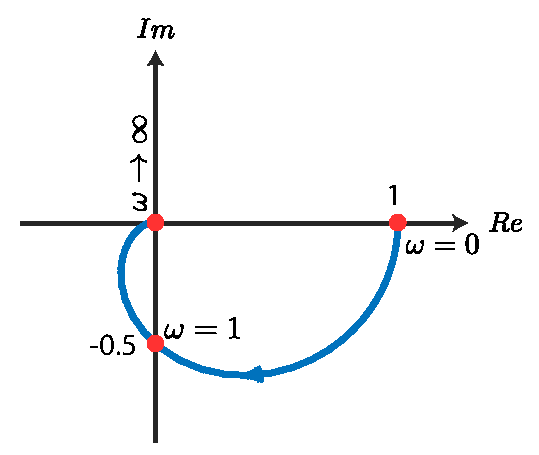
\includegraphics[width=0.5\textwidth]{polar4}
    \end{center}
  \end{minipage}

\vspace{6 pt}

Now let's draw the polar plot of  $G(s) = \frac{1}{(s+1)^3}$
%
\begin{align*}
  G(j \omega ) &= \frac{1}{ (j \omega + 1)^3 } = \frac{ (-j \omega + 1)^3 }{( \omega^2 +1 )^3 }
\\
&= \left[ \left( 1 - 3 \omega^2 \right) + j (\omega^3 - 3 \omega) \right] \frac{1}{( \omega^2 +1 )^3 }
\end{align*}
%
Some important points and associated features on the polar plot can be computed as
\begin{align*}
  \omega &\to 0 \ \Rightarrow G(j \omega) = 1
\\
 \omega &\to \sqrt{1/3} \ \Rightarrow G(j \omega) = -0.65 j 
\\
 \omega &\to \sqrt{3} \ \Rightarrow G(j \omega) = -1/4 
\\
 \omega &\to  \infty \ \Rightarrow | G(j \omega) | \to 0 \quad \& \quad \angle  [ G(j \omega) ] \to \pi/2
\end{align*}

Resultant polar plot is illustrated below

\vspace{6 pt}

  \begin{minipage}[h]{1\linewidth}
    \begin{center}
      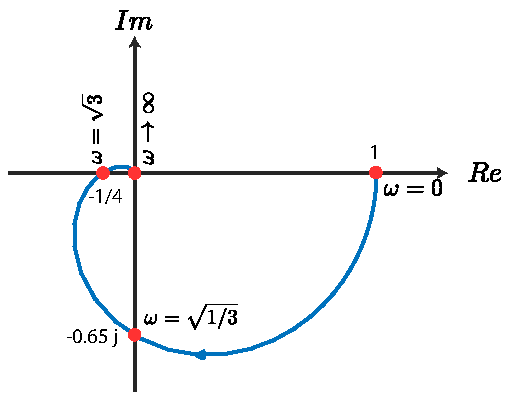
\includegraphics[width=0.6\textwidth]{polar5}
    \end{center}
  \end{minipage}

\vspace{6 pt}

% **** This ENDS THE EXAMPLES. DON'T DELETE THE FOLLOWING LINE:
\end{document}